\PassOptionsToPackage{unicode=true}{hyperref} % options for packages loaded elsewhere
\PassOptionsToPackage{hyphens}{url}
%
\documentclass[
  twoside]{article}
\usepackage{lmodern}
\usepackage{amssymb,amsmath}
\usepackage{ifxetex,ifluatex}
\ifnum 0\ifxetex 1\fi\ifluatex 1\fi=0 % if pdftex
  \usepackage[T1]{fontenc}
  \usepackage[utf8]{inputenc}
  \usepackage{textcomp} % provides euro and other symbols
\else % if luatex or xelatex
  \usepackage{unicode-math}
  \defaultfontfeatures{Scale=MatchLowercase}
  \defaultfontfeatures[\rmfamily]{Ligatures=TeX,Scale=1}
  \setmainfont[]{Verdana}
\fi
% use upquote if available, for straight quotes in verbatim environments
\IfFileExists{upquote.sty}{\usepackage{upquote}}{}
\IfFileExists{microtype.sty}{% use microtype if available
  \usepackage[]{microtype}
  \UseMicrotypeSet[protrusion]{basicmath} % disable protrusion for tt fonts
}{}
\makeatletter
\@ifundefined{KOMAClassName}{% if non-KOMA class
  \IfFileExists{parskip.sty}{%
    \usepackage{parskip}
  }{% else
    \setlength{\parindent}{0pt}
    \setlength{\parskip}{6pt plus 2pt minus 1pt}}
}{% if KOMA class
  \KOMAoptions{parskip=half}}
\makeatother
\usepackage{xcolor}
\IfFileExists{xurl.sty}{\usepackage{xurl}}{} % add URL line breaks if available
\IfFileExists{bookmark.sty}{\usepackage{bookmark}}{\usepackage{hyperref}}
\hypersetup{
  pdftitle={Latex, YAML, RMarkdown},
  pdfauthor={Fabian Koch},
  pdfborder={0 0 0},
  breaklinks=true}
\urlstyle{same}  % don't use monospace font for urls
\usepackage[margin=1in]{geometry}
\usepackage{graphicx,grffile}
\makeatletter
\def\maxwidth{\ifdim\Gin@nat@width>\linewidth\linewidth\else\Gin@nat@width\fi}
\def\maxheight{\ifdim\Gin@nat@height>\textheight\textheight\else\Gin@nat@height\fi}
\makeatother
% Scale images if necessary, so that they will not overflow the page
% margins by default, and it is still possible to overwrite the defaults
% using explicit options in \includegraphics[width, height, ...]{}
\setkeys{Gin}{width=\maxwidth,height=\maxheight,keepaspectratio}
\setlength{\emergencystretch}{3em}  % prevent overfull lines
\providecommand{\tightlist}{%
  \setlength{\itemsep}{0pt}\setlength{\parskip}{0pt}}
\setcounter{secnumdepth}{-2}
% Redefines (sub)paragraphs to behave more like sections
\ifx\paragraph\undefined\else
  \let\oldparagraph\paragraph
  \renewcommand{\paragraph}[1]{\oldparagraph{#1}\mbox{}}
\fi
\ifx\subparagraph\undefined\else
  \let\oldsubparagraph\subparagraph
  \renewcommand{\subparagraph}[1]{\oldsubparagraph{#1}\mbox{}}
\fi

% set default figure placement to htbp
\makeatletter
\def\fps@figure{htbp}
\makeatother

\setlength{\columnsep}{18pt}
\usepackage{multicol}
\newcommand{\hideFromPandoc}[1]{#1}
\hideFromPandoc{ \let\Begin\begin \let\End\end }
\definecolor{DoStat}{RGB}{184, 40, 60}
\usepackage{fancyhdr}
\pagestyle{fancy}
\fancyhf{}
\fancyhead[LE]{\itshape\nouppercase{\color{DoStat}\leftmark}}
\fancyhead[RO]{\itshape\nouppercase{\color{DoStat}\leftmark}}
\fancyfoot[LE]{\color{DoStat} \thepage \hspace{0.5cm} dortmunder\textbf{statistik}  • nr. 211 • jahresbericht 2018 • bevölkerung}
\fancyfoot[RO]{\color{DoStat} dortmunder\textbf{statistik}  • nr. 211 • jahresbericht 2018 • bevölkerung \hspace{0.5cm} \thepage}
\usepackage{booktabs}
\usepackage{longtable}
\usepackage{array}
\usepackage{multirow}
\usepackage{wrapfig}
\usepackage{float}
\usepackage{colortbl}
\usepackage{pdflscape}
\usepackage{tabu}
\usepackage{threeparttable}
\usepackage{threeparttablex}
\usepackage[normalem]{ulem}
\usepackage{makecell}
\usepackage{xcolor}

\title{Latex, YAML, RMarkdown}
\usepackage{etoolbox}
\makeatletter
\providecommand{\subtitle}[1]{% add subtitle to \maketitle
  \apptocmd{\@title}{\par {\large #1 \par}}{}{}
}
\makeatother
\subtitle{Options, packages and examples for PDF print}
\author{Fabian Koch}
\date{}

\begin{document}
\maketitle

\newpage 
\tableofcontents

\newpage

\newpage

\hypertarget{wiki}{%
\section{Wiki}\label{wiki}}

\hypertarget{packages}{%
\subsubsection{packages}\label{packages}}

\begin {multicols}{2}

\hypertarget{r---rticles}{%
\paragraph{R - rticles}\label{r---rticles}}

Templates und Vorlagen wissenschaftlicher Journals

\href{https://github.com/rstudio/rticles}{rtcles}

\hypertarget{r---ymlthis}{%
\paragraph{R - ymlthis}\label{r---ymlthis}}

package zur vereinfachten Verwendung von YAML in RMarkdown und bookdown

\href{https://cran.r-project.org/web/packages/ymlthis/vignettes/introduction-to-ymlthis.html}{Einführung}

\href{https://cran.r-project.org/web/packages/ymlthis/ymlthis.pdf}{Refrence
Manual}

\href{https://cran.r-project.org/web/packages/ymlthis/vignettes/yaml-fieldguide.html}{YAML
Field Guide}

\href{https://github.com/r-lib/ymlthis/blob/master/R/yml_latex.R}{yml\_latex.R}

\href{https://rdrr.io/github/r-lib/ymlthis/man/yml_latex_opts.html}{yml\_latex\_opts
- Set LaTeX YAML options for PDF output}

\href{https://www.rdocumentation.org/packages/ymlthis/versions/0.1.2/topics/yml_resource_files}{yml\_resource\_files
- Add external resource files to R Markdown document}

\href{https://github.com/r-lib/ymlthis/blob/master/R/yml_output.R}{yml\_output
- Capture, validate, and write output YAML}

\hypertarget{r---bookdown}{%
\paragraph{R - bookdown}\label{r---bookdown}}

Authoring Books and Technical Documents with R Markdown

Single Page Documents
\url{https://bookdown.org/yihui/bookdown/a-single-document.html}

customization
\url{https://bookdown.org/yihui/bookdown/customization.html}
\columnbreak

\hypertarget{latex-processors}{%
\paragraph{Latex processors}\label{latex-processors}}

{[}Latex
engines{]}(\url{https://tex.stackexchange.com/questions/36/differences-between-luatex-context-and-xetex}

\hypertarget{latex---multicol}{%
\paragraph{Latex - Multicol}\label{latex---multicol}}

\url{https://www.ctan.org/pkg/multicol}

\url{https://tex.stackexchange.com/questions/8683/how-do-i-force-a-column-break-in-a-multi-column-page}

\url{https://stackoverflow.com/questions/40982836/latex-multicolumn-block-in-pandoc-markdown}

Mögliche Lösungen für 2 Spalten:
\url{https://github.com/yihui/rmarkdown-cookbook/issues/19}

\url{https://stackoverflow.com/questions/34808612/how-make-2-column-layout-in-r-markdown-when-rendering-pdf}

\hypertarget{latex---koma-script}{%
\paragraph{Latex - koma Script}\label{latex---koma-script}}

package und class Sammlung \url{https://www.ctan.org/pkg/koma-script}

inkl. Fußnoten package
\url{https://ctan.org/pkg/scrlayer-scrpage?lang=de}

\hypertarget{latex---fancyhdr}{%
\paragraph{Latex - fancyhdr}\label{latex---fancyhdr}}

\href{https://ctan.org/pkg/fancyhdr?lang=de}{Kopf- und Fußzeilen}

\href{http://tug.ctan.org/tex-archive/macros/latex/contrib/fancyhdr/fancyhdr.pdf}{User
Guide}

\href{https://bookdown.org/yihui/rmarkdown-cookbook/latex-header.html}{Abschnitt
aus "bookdown}

\newpage

\hypertarget{formatierung}{%
\subsubsection{Formatierung}\label{formatierung}}

\hypertarget{seitenwechsel}{%
\paragraph{Seitenwechsel}\label{seitenwechsel}}

Latex Page Breaks
\url{https://web.archive.org/web/20100622022829/http://help-csli.stanford.edu/tex/latex-pagebreaks.shtml}

\hypertarget{text}{%
\subsubsection{Text}\label{text}}

\hypertarget{headline-1}{%
\section{Headline 1}\label{headline-1}}

\hypertarget{headline-2}{%
\subsection{Headline 2}\label{headline-2}}

\hypertarget{headline-3}{%
\subsubsection{Headline 3}\label{headline-3}}

\hypertarget{headline-4}{%
\paragraph{Headline 4}\label{headline-4}}

\hypertarget{headline-5}{%
\subparagraph{Headline 5}\label{headline-5}}

Lorem ipsum dolor sit amet, consetetur sadipscing elitr, sed diam nonumy
eirmod tempor invidunt ut labore et dolore magna aliquyam erat, sed diam
voluptua. At vero eos et accusam et justo duo dolores et ea rebum. Stet
clita kasd gubergren, no sea takimata sanctus est Lorem ipsum dolor sit
amet. Lorem ipsum dolor sit amet, consetetur sadipscing elitr, sed diam
nonumy eirmod tempor invidunt ut labore et dolore magna aliquyam erat,
sed diam voluptua.

\end {multicols}

vero eos et accusam et justo duo dolores et ea rebum. Stet clita kasd
gubergren, no sea takimata sanctus est Lorem ipsum dolor sit amet.Lorem
ipsum dolor sit amet, consetetur sadipscing elitr, sed diam nonumy
eirmod tempor invidunt ut labore et dolore magna aliquyam erat, sed diam
voluptua. At vero eos et accusam et justo duo dolores et ea rebum. Stet
clita kasd gubergren, no sea takimata sanctus est Lorem ipsum dolor sit
amet. Lorem ipsum dolor sit amet, consetetur sadipscing elitr, sed diam
nonumy eirmod tempor invidunt ut labore et dolore magna aliquyam erat,
sed diam voluptua. At vero eos et accusam et justo duo dolores et ea
rebum. Stet clita kasd gubergren, no sea takimata sanctus est Lorem
ipsum dolor sit amet.

\newpage

\hypertarget{gemischtes-1-und-2-spalten-layout}{%
\section{Gemischtes 1 und 2 Spalten
Layout}\label{gemischtes-1-und-2-spalten-layout}}

\begin {multicols}{2}

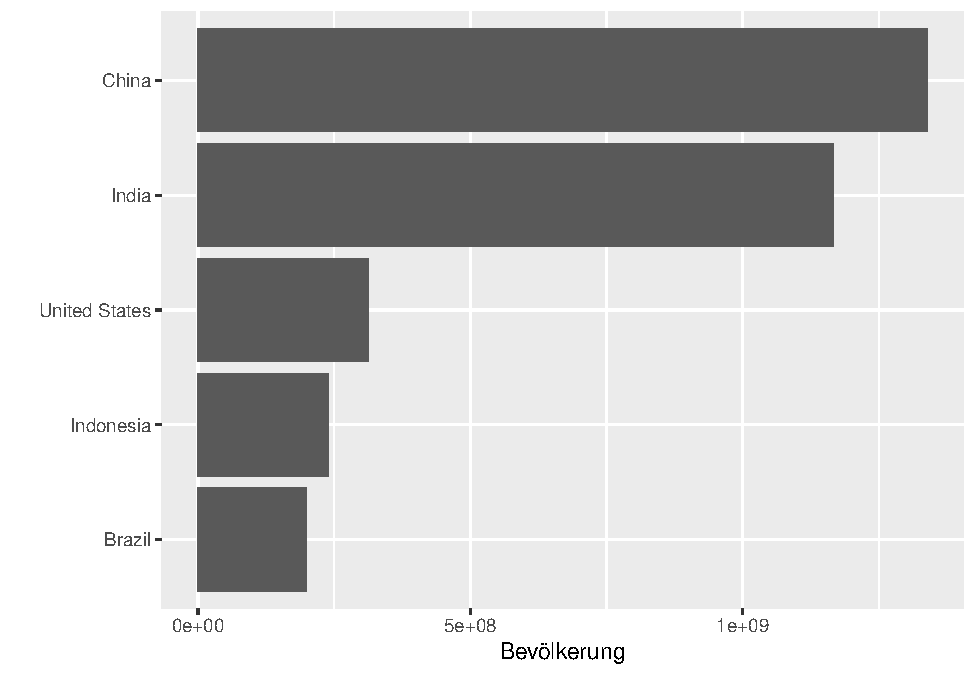
\includegraphics[width=1\linewidth]{PDF_Latex_files/figure-latex/unnamed-chunk-3-1}

Lorem ipsum dolor sit amet, consetetur sadipscing elitr, sed diam nonumy
eirmod tempor invidunt ut labore et dolore magna aliquyam erat, sed diam
voluptua. At vero eos et accusam et justo duo dolores et ea rebum. Stet
clita kasd gubergren, no sea takimata sanctus est Lorem ipsum dolor sit
amet. Lorem ipsum dolor sit amet, consetetur sadipscing elitr, sed diam
nonumy eirmod tempor invidunt ut labore et dolore magna aliquyam erat,
sed diam voluptua. At vero eos et accusam et justo duo dolores et ea
rebum. Stet clita kasd gubergren, no sea takimata sanctus est Lorem
ipsum dolor sit amet. \columnbreak

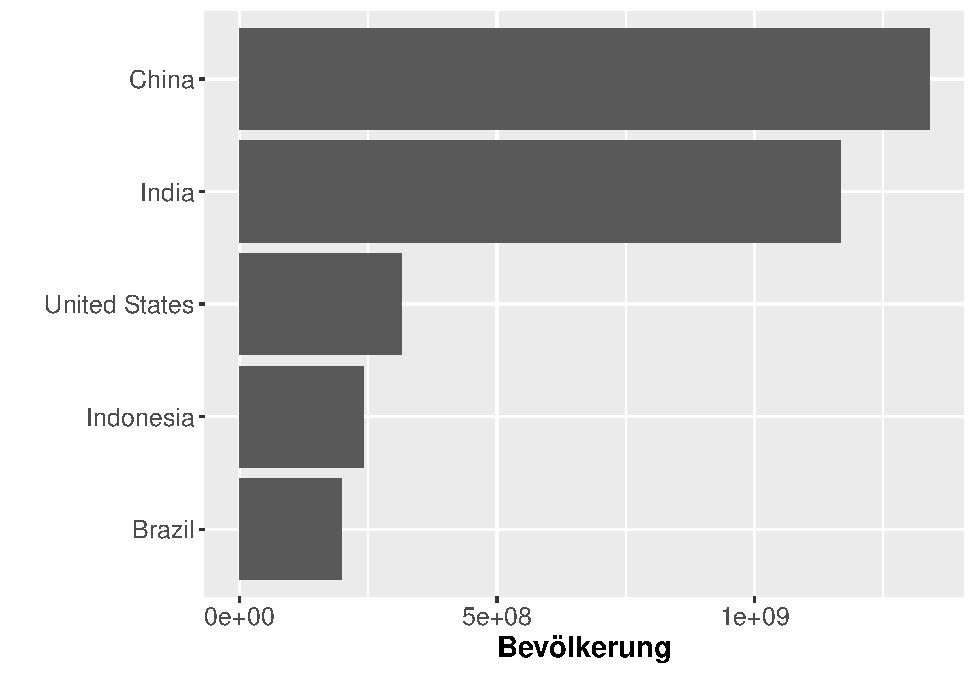
\includegraphics[width=1\linewidth]{PDF_Latex_files/figure-latex/unnamed-chunk-4-1}

Lorem ipsum dolor sit amet, consetetur sadipscing elitr, sed diam nonumy
eirmod tempor invidunt ut labore et dolore magna aliquyam erat, sed diam
voluptua. At vero eos et accusam et justo duo dolores et ea rebum. Stet
clita kasd gubergren, no sea takimata sanctus est Lorem ipsum dolor sit
amet. Lorem ipsum dolor sit amet, consetetur sadipscing elitr, sed diam
nonumy eirmod tempor invidunt ut labore et dolore magna aliquyam erat,
sed diam voluptua. At vero eos et accusam et justo duo dolores et ea
rebum. Stet clita kasd gubergren, no sea takimata sanctus est Lorem
ipsum dolor sit amet.

\end {multicols}

Lorem ipsum dolor sit amet, consetetur sadipscing elitr, sed diam nonumy
eirmod tempor invidunt ut labore et dolore magna aliquyam erat, sed diam
voluptua. At vero eos et accusam et justo duo dolores et ea rebum. Stet
clita kasd gubergren, no sea takimata sanctus est Lorem ipsum dolor sit
amet. Lorem ipsum dolor sit amet, consetetur sadipscing elitr, sed diam
nonumy eirmod tempor invidunt ut labore et dolore magna aliquyam erat,
sed diam voluptua. At vero eos et accusam et justo duo dolores et ea
rebum. Stet clita kasd gubergren, no sea takimata sanctus est Lorem
ipsum dolor sit amet.

\begin{verbatim}
## `summarise()` ungrouping output (override with `.groups` argument)
\end{verbatim}

\begin{table}[H]
\centering
\resizebox{\linewidth}{!}{
\begin{tabular}[t]{lrrrrrr}
\toprule
\multicolumn{4}{c}{ } & \multicolumn{3}{c}{Index} \\
\cmidrule(l{3pt}r{3pt}){5-7}
Kontinent & Bevölkerungsdichte & BIP (pro Kopf) & Lebenserwartung & Wohlbefinden & Ungleichheit & Happy Planet\\
\midrule
\cellcolor{gray!6}{Africa} & \cellcolor{gray!6}{60.4} & \cellcolor{gray!6}{3391.9} & \cellcolor{gray!6}{59.8} & \cellcolor{gray!6}{4.4} & \cellcolor{gray!6}{0.4} & \cellcolor{gray!6}{19.9}\\
Asia & 176.0 & 13605.7 & 71.7 & 5.1 & 0.2 & 27.9\\
\cellcolor{gray!6}{Europe} & \cellcolor{gray!6}{114.6} & \cellcolor{gray!6}{25960.5} & \cellcolor{gray!6}{77.9} & \cellcolor{gray!6}{6.1} & \cellcolor{gray!6}{0.1} & \cellcolor{gray!6}{27.2}\\
North America & 136.3 & 14725.4 & 73.9 & 6.1 & 0.2 & 32.2\\
\cellcolor{gray!6}{Oceania} & \cellcolor{gray!6}{19.4} & \cellcolor{gray!6}{13074.2} & \cellcolor{gray!6}{78.3} & \cellcolor{gray!6}{7.0} & \cellcolor{gray!6}{0.1} & \cellcolor{gray!6}{31.0}\\
\addlinespace
South America & 20.6 & 11045.6 & 74.2 & 6.3 & 0.2 & 32.3\\
\bottomrule
\end{tabular}}
\end{table}

\end{document}
